\section{Results}

We can use the uniqueness measure to understand the rate at which new ideas arrive. As we gather more and more ideas in the course of an experiment, we expect that we will see fewer ideas that are not already in our idea pool. Figure FIG shows the cumulative count of ideas as a function of the number of instances gathered in the experiment. To smooth the plot, the order in which instances were received was shuffled 100 times, and the mean of the cumulative unique idea count was taken at each step.

\begin{figure}[h!]
    \centering
    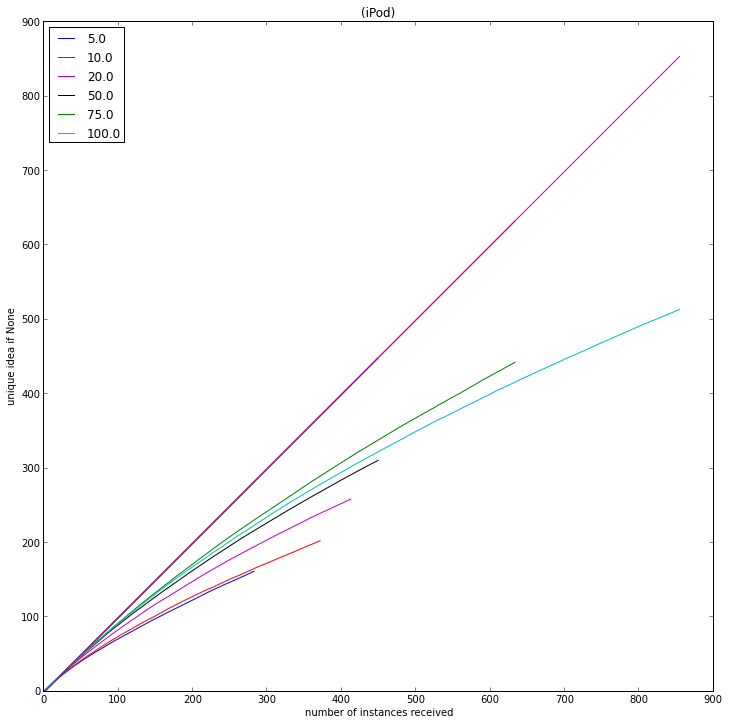
\includegraphics[width=0.9\columnwidth]{ideas_over_time}
    \caption{Cumulative idea count}
\end{figure}

The horizontal line in Figure FIG represent the idea case, in which each instance represents a different idea (i.e. every answer we receive is a new, unique idea). As expected, the rate at which ideas are gained appears to taper off.

Figure FIG more closely examines the rate, the primary property of interest. The panels, from top to bottom, are the rate at which new ideas, categories, and non-singleton categories are generated, respectively. Similar to Figure FIG, these are based on shuffling the order of instances 10000 times and taking the mean of the derivative at each point. In this case, the ideal (a 1:1:1 instance:idea:category ratio) is represented by the horizontal bar across the top of the chart.

\begin{figure}[h!]
    \centering
    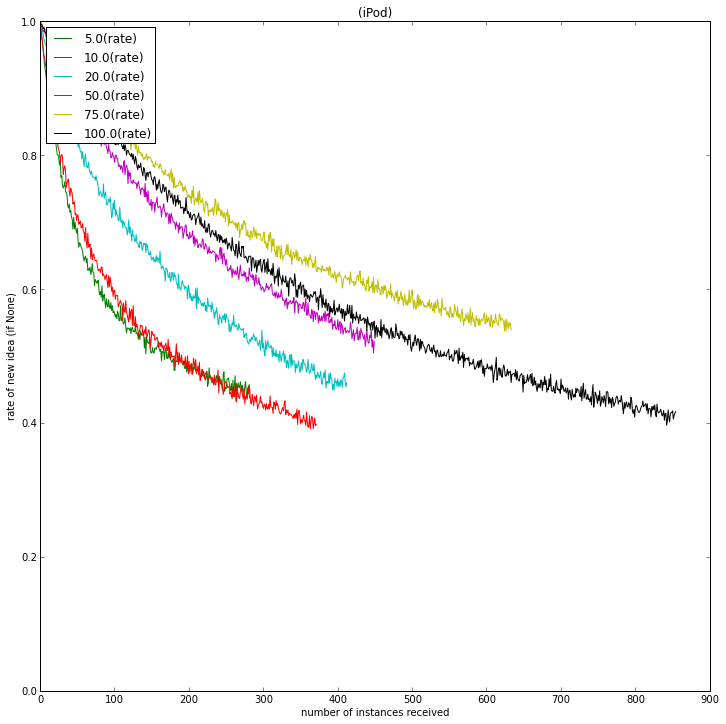
\includegraphics[width=0.7\columnwidth]{rate_new_idea_over_time}
    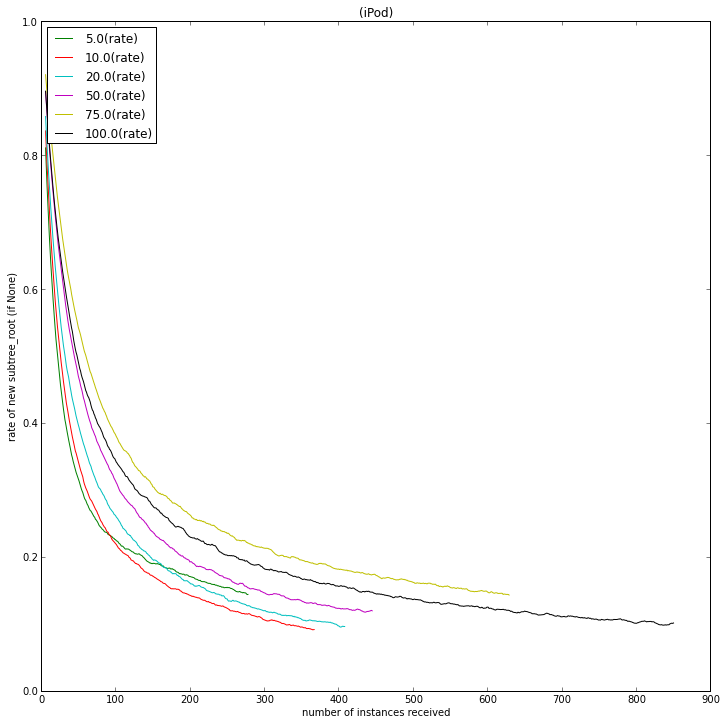
\includegraphics[width=0.7\columnwidth]{rate_new_category_over_time}
    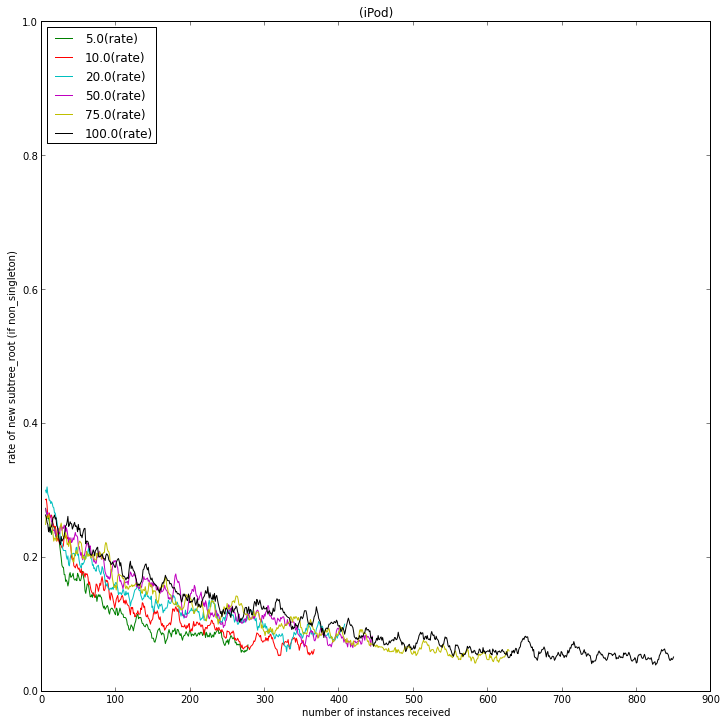
\includegraphics[width=0.7\columnwidth]{rate_new_ns_category_over_time}
    \caption{Rate of idea generation}
\end{figure}

The number of ideas, categories and non-singleton each drop off exponentially over time. It is unsurprising that the number of new categories should drop off faster than the number of new ideas, as we expect that there are fewer categories of ideas than there are individual ideas themselves.

The third panel, which shows non-singleton categories over time, tells a distinctly different story from the others. While in the idea and category plots, the height-ordering of rates of generation between categories remains generally identical, there is a point of intersection and reversal in the non-singleton category plot at around the 30 instances point. Before this point, the lower conditions actually generate new categories at a \emph{faster} rate.

In lower conditions, brainstormers will quickly offer up big, popular, non-singleton categories. Beyond the inflection point, the category pool is saturated with these low-hanging fruit, and only brainstormers tasked with generating more ideas will find the smaller category. This is a more nuanced view of the tree node/instance quartiles in Section SEC; condition 5 brainstormers cover the spectrum of category sizes while condition 100 brainstormers pull from the smaller category trees in the forest.

\subsection{Hypothesis 1}

Visually, the rate of idea, category and singleton category generation seems to trend towards 0. We tested this hypothesis...

Additionally Figure FIG indicates that there is some effect of number of ideas requested on the rate of generation. Generally, conditions with more requested responses generated ideas and categories at a higher rate. We tested this...

\subsection{Originality}

We were also interested in the effect of the number requested condition on originality. Originality, as measured by o-scores at both the category and idea level, is compared cross condition in figure FIG. Some stat tests here...

\begin{figure}[h]
    \centering
    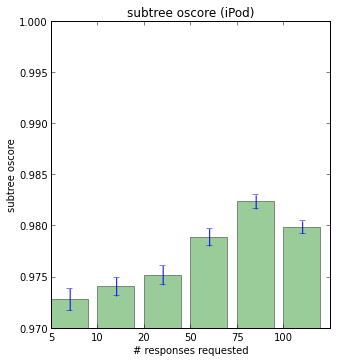
\includegraphics[width=0.9\columnwidth]{subtree_oscore}
    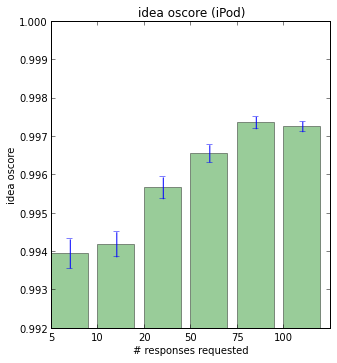
\includegraphics[width=0.9\columnwidth]{idea_oscore}
    \caption{Error bars are standard error}
\end{figure}

The more ideas requested, the more original the ideas produced. This provides support for the findings of Parnes et al \cite{parnes_effects_1961}, namely that more original ideas are found in extended idea generation events. This finding will be examined in the next section.




\subsection{Brainstorming Runs}

The large, experiment-scale trends we describe above are composed of ideas generated in many individual brainstorming runs.

\subsubsection{Originality}

In the previous section, we showed that originality at both the idea and category tree level rose as the number of responses solicited increased. Parnes et al fround that ideas generated in the latter half of a brainstorming session were rated more original in colocated, cotemporal idea generation groups \cite{parnes_effects_1961}. We hypothesize that we should see a difference in idea and category oscore as a function of position in the brainstorming run, with later ideas performing better. Figure FIG presents the mean oscroe ratings on this scale.

\begin{figure}[h]
    \centering
    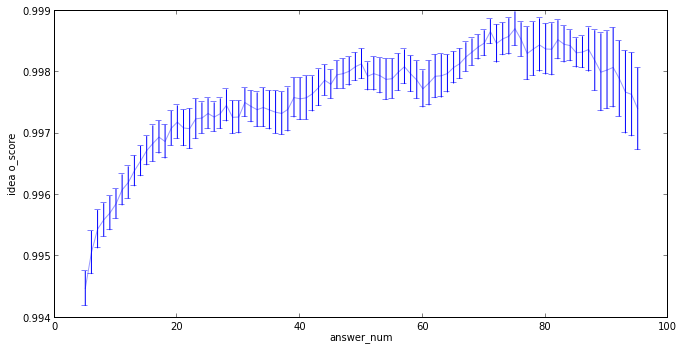
\includegraphics[width=0.9\columnwidth]{run_idea_oscore}
    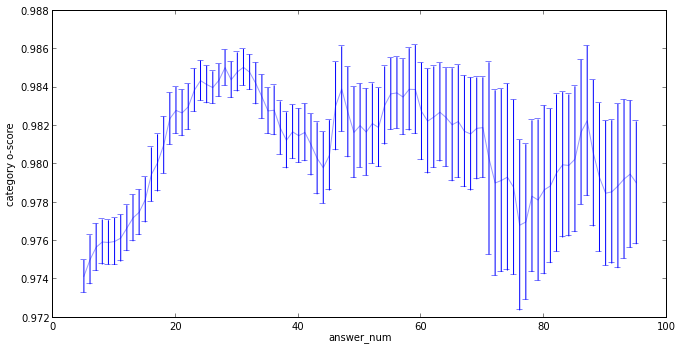
\includegraphics[width=0.9\columnwidth]{run_category_oscore}
    \caption{Error bars are standard error}
\end{figure}

There appears to be a clear, uniform increase in originality on both measures through the 20th idea, at which point originality peters out, or, in the case of category o-score, becomes highly variant. We tested the hypothesis that ideas were less creative after the 20th...

Thus, we confirm Parnes et al's prior result: later ideas are more original than those early in the run. Furthermore, we identify 20 ideas as a key inflection point past which participants have realiably exhausted their supply of readily available ideas and begin generating their most original ideas.

\subsubsection{Generality}

Similarly, generatility was found to decrease as the number of ideas requested increased. Figure FIG shows generality over the course of a brainstorming run.

\begin{figure}[h]
    \centering
    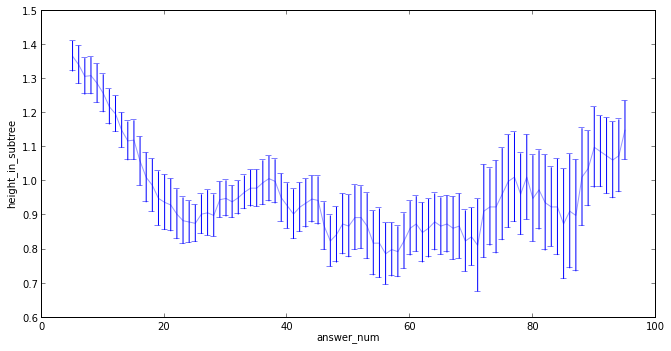
\includegraphics[width=0.9\columnwidth]{run_height_in_subtree}
    \caption{Error bars are standard error}
\end{figure}

Unsurprisingly, generality performs inversely to originality - the most general ideas are the least original. Also like originality, participants seem to exhaust their supply of general ideas by around the 20th idea, at which point they produce ideas at a fairly uniform generality. We tested this...

\subsubsection{SIAM hypotheses}

\cite{nijstad_how_2006}